
\chapter{Ugeopgave 2}
\label{cha:ugeopgave-2}

Denne ugeopgave besk�ftiger sig med forskellige m�der at lave det
virtuelle kamera, samt at g�re os bekvemme med at �ndre p� parametrene
til kamerafunktionerne.

\section{Del 1}
\label{sec:del-1:-isometri}

I denne opgave skulle der laves et isometri-\emph{view}. Dette blev
gjort ved at s�tte �jepunktet i $(2,2,2)$, da kameraet dermed kigger
``korrekt'' skr�t nedad mod �jepunktet i $(0,0,0)$. Resultatet af
dette, med op-vektoren pegende i z-aksens retning, ses p� figur
\ref{fig:2-1}.


\begin{figure}[hp]
\centering
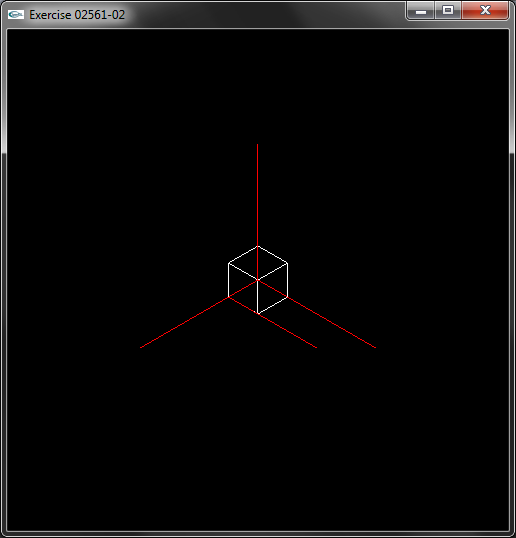
\includegraphics[width=8cm]{../exercise2/screenshots/part1.png}
\caption{Isometrisk view}
\label{fig:2-1}
\end{figure}

\section{Del 2}
\label{sec:del-2:-viewing}

Viewing transformationen kan generelt opn�s med et antal rotationer og
evt. en translatering. Idet vi g�r brug af et ortografisk view, har vi
dog ikke brug for at translatere, da denne operation ikke bestemmer
st�rrelsen af objekterne i scenen, men blot om de bliver
\emph{clipped} eller ej, og vores ops�tning g�r at terningen ikke kan
risikere at blive \emph{clipped} v�k.

For at opn� det samme billede som med \texttt{gluLookAt}, har vi behov
for f�lgende operationer:

\begin{itemize}
\item $-90 \degree$ rotation om x-aksen
\item $-135 \degree$ rotation om y-aksen
\item $35.26 \degree$ rotation om x-aksen\footnote{Se Angel s. 247 for forklaring} 
\end{itemize}

Dermed er vores matricer som f�lger:

\begin{align*}
  \mathbf{R}_1 = &
    \begin{bmatrix}
      1 & 0 & 0 & 0 \\
      0 & cos -90 \degree & -sin -90 \degree & 0 \\
      0 & sin -90 \degree & cos -90 \degree & 0 \\
      0 & 0 & 0 & 1
    \end{bmatrix} \\
  \mathbf{R}_2 = &
    \begin{bmatrix}
      cos -135 \degree & 0 & sin -135 \degree & 0 \\
      0 & 1 & 0 & 0 \\
      -sin -135 \degree & 0 & cos -135 \degree & 0 \\
      0 & 0 & 0 & 1
    \end{bmatrix} \\
  \mathbf{R}_3 = &
    \begin{bmatrix}
      1 & 0 & 0 & 0 \\
      0 & cos 35.26 \degree & -sin 35.26 \degree & 0 \\
      0 & sin 35.26 \degree & cos 35.26 \degree & 0 \\
      0 & 0 & 0 & 1
    \end{bmatrix} \\
\end{align*}

Resultatet af vores manuelle ops�tning af kameraet kan ses p� figur
\ref{fig:2-2}. Som det kan ses er den identisk med figur \ref{fig:2-1}

\begin{figure}[hp]
\centering
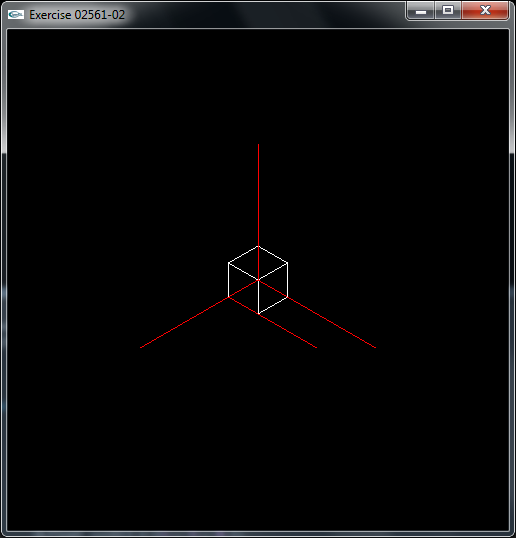
\includegraphics[width=8cm]{../exercise2/screenshots/part2.png}
\caption{Manuel ops�tning af kamera}
\label{fig:2-2}
\end{figure}

\section{Del 3}
\label{sec:del-3}

Denne del er s� vidt vi kan se allerede l�st i forbindelse med
forg�ende delopgave.


%%% Local Variables: 
%%% mode: latex
%%% TeX-master: "report_main"
%%% End: 
